\documentclass[11pt]{article}

\usepackage[letterpaper,margin=1in]{geometry}
\usepackage{lmodern}
\usepackage[T1]{fontenc}
\usepackage{microtype}
\usepackage{amsmath,amssymb}
\usepackage{booktabs}
\usepackage{tabularx}
\usepackage{array}
\usepackage{enumitem}
\usepackage{xcolor}
\usepackage{tikz}
\usepackage{pgfplots}
\usepackage[most]{tcolorbox}
\usepackage{hyperref}
\usepackage{fancyhdr}
\usepackage{lastpage}

\pgfplotsset{compat=1.18}
\usetikzlibrary{arrows.meta,positioning,calc,fit,shapes.geometric,decorations.pathreplacing,backgrounds}

\definecolor{deepblue}{HTML}{1F4E79}
\definecolor{lightblue}{HTML}{EAF3FA}
\definecolor{softgreen}{HTML}{EAF7EA}
\definecolor{softorange}{HTML}{FFF3E0}
\definecolor{softpurple}{HTML}{F0ECFA}
\definecolor{softred}{HTML}{FDEDED}
\definecolor{graytext}{HTML}{555555}

\hypersetup{
  colorlinks=true,
  linkcolor=deepblue,
  urlcolor=deepblue,
  citecolor=deepblue,
  pdftitle={A Friendly Tutorial on Bayesian Inference},
  pdfauthor={OpenAI}
}

\pagestyle{fancy}
\fancyhf{}
\lhead{Bayesian Inference Tutorial}
\rhead{High-school friendly}
\cfoot{\thepage\ of \pageref{LastPage}}
\renewcommand{\headrulewidth}{0.4pt}
\setlength{\headheight}{14pt}

\setlength{\parindent}{0pt}
\setlength{\parskip}{0.55em}
\renewcommand{\arraystretch}{1.22}

\newtcolorbox{bigidea}{
  enhanced, breakable,
  colback=lightblue,
  colframe=deepblue,
  title=Big idea,
  fonttitle=\bfseries,
  arc=2mm,
  boxrule=0.8pt
}

\newtcolorbox{warningbox}{
  enhanced, breakable,
  colback=softred,
  colframe=red!55!black,
  title=Common confusion,
  fonttitle=\bfseries,
  arc=2mm,
  boxrule=0.8pt
}

\newtcolorbox{examplebox}{
  enhanced, breakable,
  colback=softgreen,
  colframe=green!45!black,
  title=Example,
  fonttitle=\bfseries,
  arc=2mm,
  boxrule=0.8pt
}

\newtcolorbox{recipebox}{
  enhanced, breakable,
  colback=softorange,
  colframe=orange!60!black,
  title=Recipe,
  fonttitle=\bfseries,
  arc=2mm,
  boxrule=0.8pt
}

\newtcolorbox{checkbox}{
  enhanced, breakable,
  colback=softpurple,
  colframe=purple!55!black,
  title=Assumption check,
  fonttitle=\bfseries,
  arc=2mm,
  boxrule=0.8pt
}

\newcommand{\data}{\text{data}}
\newcommand{\prior}{\text{prior}}
\newcommand{\likelihood}{\text{likelihood}}
\newcommand{\posterior}{\text{posterior}}

\title{\vspace{-1cm}\Huge A Friendly Tutorial on Bayesian Inference\\[0.2cm]
\Large What to model, what hyperparameters are, and where the assumptions are}
\author{Written for a high school student with limited statistics background}
\date{}

\begin{document}
\pagenumbering{roman}
\maketitle
\thispagestyle{empty}

\begin{center}
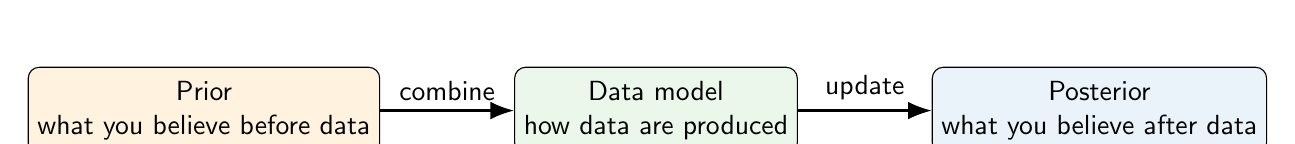
\begin{tikzpicture}[node distance=1.7cm, every node/.style={font=\sffamily}]
  \node[draw, rounded corners, fill=softorange, minimum width=3.0cm, minimum height=1.1cm, align=center] (prior) {Prior\\what you believe before data};
  \node[draw, rounded corners, fill=softgreen, right=of prior, minimum width=3.0cm, minimum height=1.1cm, align=center] (data) {Data model\\how data are produced};
  \node[draw, rounded corners, fill=lightblue, right=of data, minimum width=3.0cm, minimum height=1.1cm, align=center] (post) {Posterior\\what you believe after data};
  \draw[-{Latex[length=3mm]}, thick] (prior) -- node[above]{combine} (data);
  \draw[-{Latex[length=3mm]}, thick] (data) -- node[above]{update} (post);
\end{tikzpicture}
\end{center}

\begin{bigidea}
Bayesian inference is a way to update uncertainty. You start with a believable range of possibilities, use data to rule some possibilities up or down, and end with an updated range of possibilities.
\end{bigidea}

\vfill
\tableofcontents
\newpage
\pagenumbering{arabic}

\section{The main question: what is Bayesian inference?}

Suppose you are not sure about something. Maybe a coin is fair, maybe a basketball player makes about 70\% of free throws, or maybe a science measurement has a small error. Bayesian inference gives a language for saying:

\begin{center}
\Large
\[\text{belief before seeing data} + \text{information from data} = \text{belief after seeing data}.\]
\end{center}

The word \emph{belief} here does not mean a random guess. It means a probability distribution that describes uncertainty. Bayesian inference is especially useful when the answer is not just one number, but a range of plausible values.

\begin{bigidea}
The main output of Bayesian inference is usually a \textbf{posterior distribution}. It tells you which values are still plausible after seeing the data, and how plausible they are relative to each other.
\end{bigidea}

\subsection*{A simple everyday picture}

Imagine a mystery bag contains red and blue candies. You cannot see inside the bag. You reach in, pull out 10 candies one at a time, write down the colors, and put each candy back. You want to know the fraction of red candies in the bag.

The unknown fraction of red candies is a number between 0 and 1. Call it $p$.

\begin{itemize}[leftmargin=1.5em]
  \item If $p=0$, the bag has no red candies.
  \item If $p=0.5$, the bag is half red.
  \item If $p=1$, the bag is all red.
\end{itemize}

Before collecting data, you might think many values of $p$ are possible. After seeing many red candies, larger values of $p$ become more plausible. After seeing many blue candies, smaller values of $p$ become more plausible.

\section{The four important words}

Bayesian inference often feels confusing because several different things are called ``models'' or ``parameters.'' This table separates the ideas.

\begin{center}
\begin{tabularx}{\textwidth}{>{\bfseries}p{0.20\textwidth} X X}
\toprule
Word & Meaning & In the candy-bag example \\
\midrule
Data & The observations you actually saw. & The 10 candy colors you recorded. \\
Parameter & An unknown quantity you want to learn. & $p$, the fraction of red candies in the bag. \\
Prior & Your uncertainty about the parameter before seeing the new data. & A probability distribution over possible values of $p$ before sampling candies. \\
Likelihood & A model for how likely the data would be if the parameter had a particular value. & If $p=0.7$, how likely is it to see 8 red candies out of 10? \\
Posterior & Your uncertainty about the parameter after seeing the data. & A new probability distribution over $p$ after observing the 10 candies. \\
Hyperparameter & A setting that controls the shape of another distribution, often a prior. & Numbers like $\alpha$ and $\beta$ that control the prior distribution for $p$. \\
\bottomrule
\end{tabularx}
\end{center}

\begin{warningbox}
A \textbf{parameter} is usually an unknown thing inside the real-world process. A \textbf{hyperparameter} is usually a number that controls a distribution for a parameter. But these names depend on the level of the model. In a bigger model, a hyperparameter can become a parameter too.
\end{warningbox}

\section{Bayes' rule in one line}

Bayesian inference is based on Bayes' rule:

\begin{equation}
\boxed{\displaystyle
P(\theta \mid \data) = \frac{P(\data \mid \theta)P(\theta)}{P(\data)}
}
\end{equation}

Here $\theta$ is a common symbol for an unknown parameter. It is pronounced ``theta.''

The equation says:

\begin{equation}
\boxed{\displaystyle
\posterior = \frac{\likelihood \times \prior}{\text{evidence}}
}
\end{equation}

The denominator $P(\data)$ is called the \textbf{evidence}. Its job is to make the posterior probabilities add up to 1, or make the posterior density have total area 1. When comparing two possible parameter values, you can often think:

\begin{equation}
\posterior \propto \likelihood \times \prior.
\end{equation}

The symbol $\propto$ means ``is proportional to.'' In words: first multiply prior by likelihood, then rescale so the total is 1.

\begin{center}
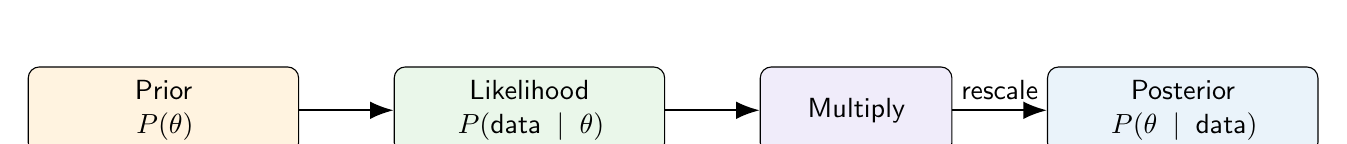
\begin{tikzpicture}[node distance=1.2cm, every node/.style={font=\sffamily}]
  \node[draw, rounded corners, fill=softorange, text width=3.2cm, align=center, minimum height=1.1cm] (a) {Prior\\$P(\theta)$};
  \node[draw, rounded corners, fill=softgreen, text width=3.2cm, align=center, minimum height=1.1cm, right=of a] (b) {Likelihood\\$P(\data\mid\theta)$};
  \node[draw, rounded corners, fill=softpurple, text width=2.2cm, align=center, minimum height=1.1cm, right=of b] (c) {Multiply};
  \node[draw, rounded corners, fill=lightblue, text width=3.2cm, align=center, minimum height=1.1cm, right=of c] (d) {Posterior\\$P(\theta\mid\data)$};
  \draw[-{Latex[length=3mm]}, thick] (a) -- (b);
  \draw[-{Latex[length=3mm]}, thick] (b) -- (c);
  \draw[-{Latex[length=3mm]}, thick] (c) -- node[above]{rescale} (d);
\end{tikzpicture}
\end{center}

\section{Tiny example: two possible coins}

Let us start with a version that uses only arithmetic. Suppose there are two possible coins:

\begin{itemize}[leftmargin=1.5em]
  \item Coin A is fair: $p=0.5$ chance of heads.
  \item Coin B is heads-biased: $p=0.8$ chance of heads.
\end{itemize}

You do not know which coin you have. Before flipping, you think they are equally likely:

\[
P(A)=0.5, \qquad P(B)=0.5.
\]

You flip the mystery coin 4 times and see 3 heads and 1 tail.

\subsection*{Step 1: compute likelihoods}

If the coin has heads probability $p$, the probability of exactly 3 heads in 4 flips is:

\[
\binom{4}{3}p^3(1-p).
\]

For Coin A:

\[
P(3H,1T \mid A)=\binom{4}{3}(0.5)^3(0.5)=0.25.
\]

For Coin B:

\[
P(3H,1T \mid B)=\binom{4}{3}(0.8)^3(0.2)=0.4096.
\]

The data are more likely if the coin is biased toward heads.

\subsection*{Step 2: multiply by prior}

\begin{center}
\begin{tabular}{lccc}
\toprule
Possible coin & Prior & Likelihood & Unnormalized posterior \\
\midrule
Coin A: $p=0.5$ & $0.5$ & $0.25$ & $0.125$ \\
Coin B: $p=0.8$ & $0.5$ & $0.4096$ & $0.2048$ \\
\bottomrule
\end{tabular}
\end{center}

These unnormalized posterior values do not add up to 1. Their sum is:

\[
0.125+0.2048=0.3298.
\]

\subsection*{Step 3: rescale}

\[
P(A\mid \data)=\frac{0.125}{0.3298}\approx 0.379,
\]

\[
P(B\mid \data)=\frac{0.2048}{0.3298}\approx 0.621.
\]

\begin{bigidea}
After seeing 3 heads in 4 flips, Coin B becomes more plausible, but Coin A is not impossible. Bayesian inference usually changes degrees of belief instead of making an all-or-nothing decision.
\end{bigidea}

\section{What exactly should have a model?}

This is one of the most important questions.

A Bayesian model usually has two parts:

\begin{equation}
\boxed{\displaystyle
P(\data, \theta)=P(\data\mid\theta)P(\theta)
}
\end{equation}

This is called a \textbf{joint model} because it describes the data and the unknown parameter together.

\subsection*{Part 1: model the data-gathering process}

You need a model for how the data could have been generated. This is the likelihood $P(\data\mid\theta)$.

For coin flips, a simple data model says:

\begin{itemize}[leftmargin=1.5em]
  \item Every flip has the same probability $p$ of heads.
  \item Flips are independent, meaning one flip does not affect the next.
  \item The result of each flip is either heads or tails.
\end{itemize}

Those are assumptions. They may be reasonable for a coin, but not for every real situation.

\subsection*{Part 2: model your uncertainty about unknowns}

You also need a prior $P(\theta)$ for unknown quantities you want to learn.

For a coin, the unknown is $p$, the chance of heads. A prior for $p$ says which values of $p$ you thought were plausible before seeing the new flips.

\begin{recipebox}
A practical rule:
\begin{enumerate}[leftmargin=1.5em]
  \item Write down the quantity you want to learn. This becomes a parameter.
  \item Write down how the data would be produced if that parameter were known. This is the likelihood.
  \item Write down your uncertainty about the parameter before seeing the data. This is the prior.
  \item Use Bayes' rule to update from prior to posterior.
\end{enumerate}
\end{recipebox}

\subsection*{Should the observed data itself have a prior?}

Usually, no. Once data are observed, they are fixed facts. But before observing them, the model treats them as possible random outcomes. That is what the likelihood does.

For example, after you see the sequence

\[
H,H,T,H,T,H,H,H,
\]

that exact sequence is no longer uncertain. But the model asks: ``If $p$ had been 0.6, how surprising would this sequence have been? If $p$ had been 0.8, how surprising would it have been?''

\section{The coin model in pictures}

Let $p$ be the unknown chance of heads. Each flip depends on $p$.

\begin{center}
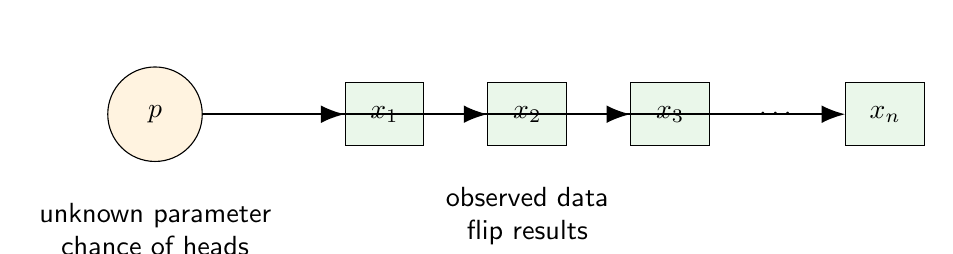
\begin{tikzpicture}[node distance=1.5cm, every node/.style={font=\sffamily}]
  \node[circle, draw, fill=softorange, minimum size=1.2cm] (p) {$p$};
  \node[rectangle, draw, fill=softgreen, minimum width=1.0cm, minimum height=0.8cm, right=1.8cm of p] (x1) {$x_1$};
  \node[rectangle, draw, fill=softgreen, minimum width=1.0cm, minimum height=0.8cm, right=0.8cm of x1] (x2) {$x_2$};
  \node[rectangle, draw, fill=softgreen, minimum width=1.0cm, minimum height=0.8cm, right=0.8cm of x2] (x3) {$x_3$};
  \node[right=0.5cm of x3] (dots) {$\cdots$};
  \node[rectangle, draw, fill=softgreen, minimum width=1.0cm, minimum height=0.8cm, right=0.5cm of dots] (xn) {$x_n$};
  \draw[-{Latex[length=3mm]}, thick] (p) -- (x1);
  \draw[-{Latex[length=3mm]}, thick] (p) -- (x2);
  \draw[-{Latex[length=3mm]}, thick] (p) -- (x3);
  \draw[-{Latex[length=3mm]}, thick] (p) -- (xn);
  \node[below=0.4cm of p, align=center, text width=3cm] {unknown parameter\\chance of heads};
  \node[below=0.4cm of x2, align=center, text width=4.4cm] {observed data\\flip results};
\end{tikzpicture}
\end{center}

The arrows mean that the flip results are modeled as depending on $p$. The arrows do not mean $p$ physically pushes the coin. They mean that if we knew $p$, we could calculate probabilities for the flip results.

\section{A continuous prior: the Beta distribution}

For a coin, $p$ can be any number from 0 to 1. A convenient prior for $p$ is called a \textbf{Beta distribution}. It has two hyperparameters, usually written as $\alpha$ and $\beta$:

\[
p \sim \operatorname{Beta}(\alpha,\beta).
\]

Read this as: ``$p$ is modeled as coming from a Beta distribution with hyperparameters $\alpha$ and $\beta$.''

The Beta distribution is useful because it is a flexible family of shapes on the interval from 0 to 1.

\begin{center}
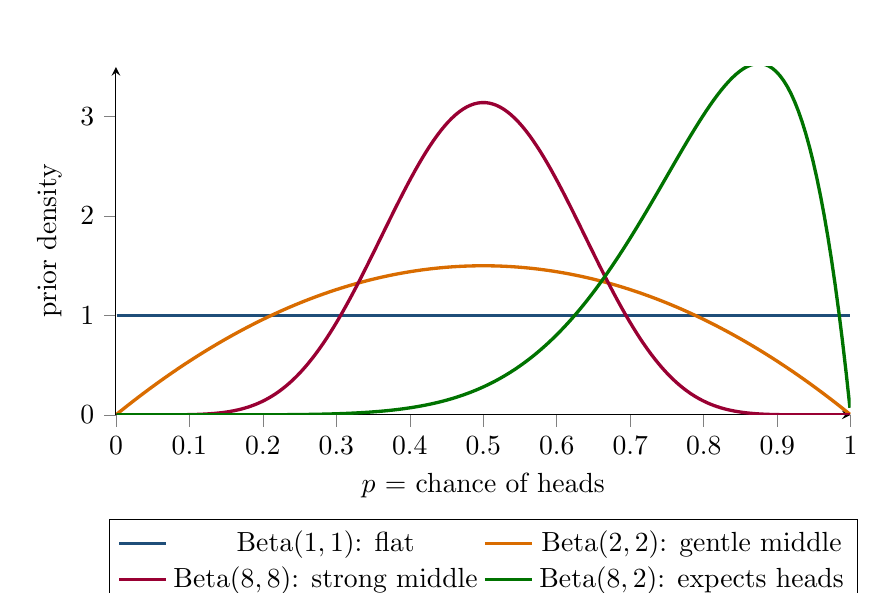
\begin{tikzpicture}
\begin{axis}[
  width=0.9\textwidth,
  height=6cm,
  xmin=0, xmax=1,
  ymin=0, ymax=3.5,
  axis lines=left,
  xlabel={$p$ = chance of heads},
  ylabel={prior density},
  legend style={at={(0.5,-0.30)},anchor=north,legend columns=2},
  tick align=outside,
  domain=0.001:0.999,
  samples=200
]
\addplot[very thick, deepblue] {1};
\addlegendentry{$\operatorname{Beta}(1,1)$: flat}
\addplot[very thick, orange!85!black] {6*x*(1-x)};
\addlegendentry{$\operatorname{Beta}(2,2)$: gentle middle}
\addplot[very thick, purple!80!black] {51480*x^7*(1-x)^7};
\addlegendentry{$\operatorname{Beta}(8,8)$: strong middle}
\addplot[very thick, green!45!black] {72*x^7*(1-x)};
\addlegendentry{$\operatorname{Beta}(8,2)$: expects heads}
\end{axis}
\end{tikzpicture}
\end{center}

\begin{bigidea}
For a Beta prior, $\alpha$ and $\beta$ are \textbf{hyperparameters}. They are not the coin's chance of heads. They control the shape of your prior belief about the coin's chance of heads.
\end{bigidea}

\subsection*{Pseudo-count intuition}

A useful rough interpretation is:

\begin{equation}
\operatorname{Beta}(\alpha,\beta) \quad \text{acts a bit like} \quad (\alpha-1) \text{ prior heads and } (\beta-1) \text{ prior tails.}
\end{equation}

This is only an intuition, but it helps.

\begin{center}
\begin{tabular}{lll}
\toprule
Prior & Informal meaning & Shape \\
\midrule
$\operatorname{Beta}(1,1)$ & No pseudo-counts & Flat from 0 to 1 \\
$\operatorname{Beta}(2,2)$ & 1 pseudo-head, 1 pseudo-tail & Mildly favors values near 0.5 \\
$\operatorname{Beta}(8,8)$ & 7 pseudo-heads, 7 pseudo-tails & Strongly favors values near 0.5 \\
$\operatorname{Beta}(8,2)$ & 7 pseudo-heads, 1 pseudo-tail & Favors large values of $p$ \\
\bottomrule
\end{tabular}
\end{center}

\section{Updating a Beta prior with coin data}

Suppose your prior is:

\[
p \sim \operatorname{Beta}(2,2).
\]

Then you flip the coin 8 times and see 6 heads and 2 tails.

For this model, the update is especially simple:

\begin{equation}
\boxed{\displaystyle
\operatorname{Beta}(\alpha,\beta) \quad + \quad H \text{ heads and } T \text{ tails}
\quad \Longrightarrow \quad
\operatorname{Beta}(\alpha+H,\beta+T).
}
\end{equation}

So:

\[
\operatorname{Beta}(2,2)+6H+2T = \operatorname{Beta}(8,4).
\]

\begin{center}
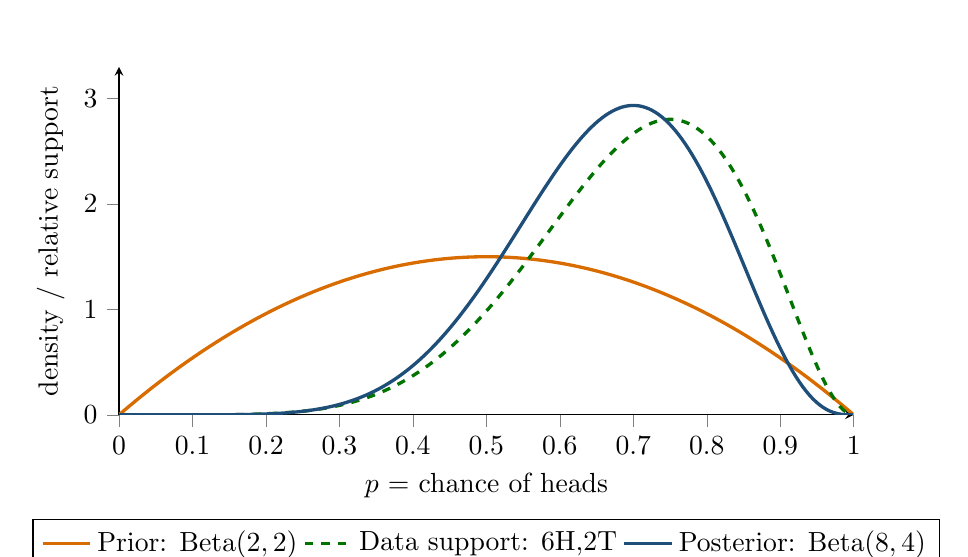
\begin{tikzpicture}
\begin{axis}[
  width=0.9\textwidth,
  height=6cm,
  xmin=0, xmax=1,
  ymin=0, ymax=3.3,
  axis lines=left,
  xlabel={$p$ = chance of heads},
  ylabel={density / relative support},
  legend style={at={(0.5,-0.30)},anchor=north,legend columns=3},
  tick align=outside,
  domain=0.001:0.999,
  samples=220
]
\addplot[very thick, orange!85!black] {6*x*(1-x)};
\addlegendentry{Prior: $\operatorname{Beta}(2,2)$}
\addplot[very thick, green!45!black, dashed] {252*x^6*(1-x)^2};
\addlegendentry{Data support: 6H,2T}
\addplot[very thick, deepblue] {1320*x^7*(1-x)^3};
\addlegendentry{Posterior: $\operatorname{Beta}(8,4)$}
\end{axis}
\end{tikzpicture}
\end{center}

The posterior is centered closer to the data than the prior was. The data alone suggest $6/8=0.75$. The prior $\operatorname{Beta}(2,2)$ gently pulls the answer back toward 0.5. The posterior mean is:

\[
\frac{8}{8+4}=\frac{8}{12}\approx 0.667.
\]

This does not mean ``the true $p$ is definitely 0.667.'' It means that after combining this prior and this data, the posterior distribution has its average at about 0.667.

\section{Why use a distribution instead of one best number?}

Suppose two students estimate a coin's chance of heads.

\begin{center}
\begin{tabular}{lcc}
\toprule
Student & Data seen & Best estimate $H/n$ \\
\midrule
Student 1 & 6 heads out of 8 flips & 0.75 \\
Student 2 & 60 heads out of 80 flips & 0.75 \\
\bottomrule
\end{tabular}
\end{center}

Both best estimates are 0.75. But Student 2 should be more confident because 80 flips are more information than 8 flips.

A posterior distribution can show this difference: many flips make the posterior narrower.

\begin{center}
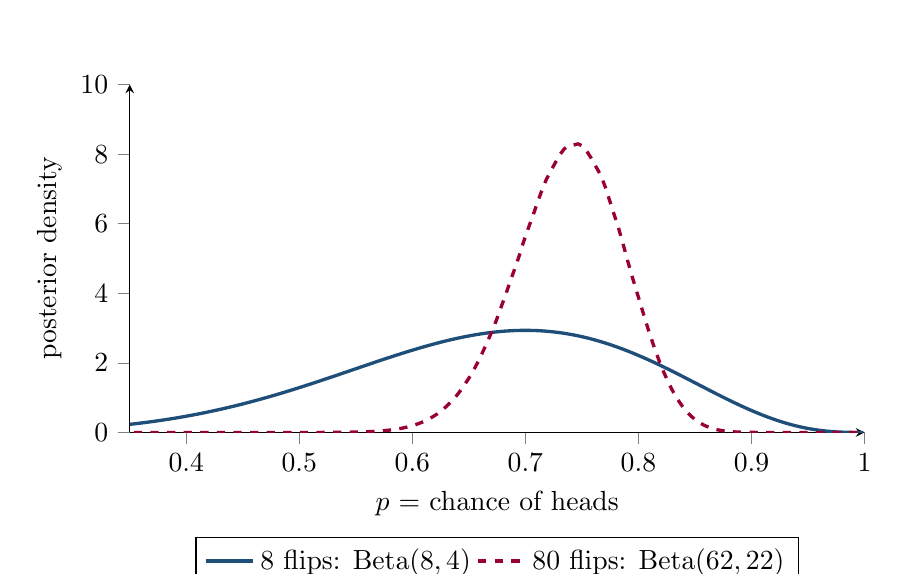
\begin{tikzpicture}
\begin{axis}[
  width=0.9\textwidth,
  height=6cm,
  xmin=0.35, xmax=1,
  ymin=0, ymax=10,
  axis lines=left,
  xlabel={$p$ = chance of heads},
  ylabel={posterior density},
  legend style={at={(0.5,-0.30)},anchor=north,legend columns=2},
  tick align=outside,
  domain=0.001:0.999,
  samples=250
]
\addplot[very thick, deepblue] {1320*x^7*(1-x)^3};
\addlegendentry{8 flips: $\operatorname{Beta}(8,4)$}
\addplot[very thick, purple!80!black, dashed] {exp(48.77394710910519 + 61*ln(x) + 21*ln(1-x))};
\addlegendentry{80 flips: $\operatorname{Beta}(62,22)$}
\end{axis}
\end{tikzpicture}
\end{center}

The tall narrow curve means the values are more concentrated. More data usually makes the posterior narrower, but only if the model assumptions are reasonable.

\section{Hyperparameters: what are they really?}

Hyperparameters are settings that control another part of the model.

In the coin model:

\[
p \sim \operatorname{Beta}(\alpha,\beta),
\]

$p$ is the parameter we are trying to learn. The numbers $\alpha$ and $\beta$ control the prior distribution for $p$. So $\alpha$ and $\beta$ are hyperparameters.

\begin{center}
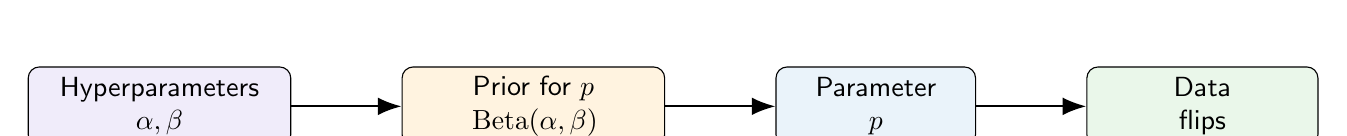
\begin{tikzpicture}[node distance=1.4cm, every node/.style={font=\sffamily}]
  \node[draw, rounded corners, fill=softpurple, text width=3.1cm, align=center, minimum height=1.0cm] (hyper) {Hyperparameters\\$\alpha,\beta$};
  \node[draw, rounded corners, fill=softorange, text width=3.1cm, align=center, minimum height=1.0cm, right=of hyper] (priornode) {Prior for $p$\\$\operatorname{Beta}(\alpha,\beta)$};
  \node[draw, rounded corners, fill=lightblue, text width=2.3cm, align=center, minimum height=1.0cm, right=of priornode] (param) {Parameter\\$p$};
  \node[draw, rounded corners, fill=softgreen, text width=2.7cm, align=center, minimum height=1.0cm, right=of param] (obs) {Data\\flips};
  \draw[-{Latex[length=3mm]}, thick] (hyper) -- (priornode);
  \draw[-{Latex[length=3mm]}, thick] (priornode) -- (param);
  \draw[-{Latex[length=3mm]}, thick] (param) -- (obs);
\end{tikzpicture}
\end{center}

\subsection*{Are hyperparameters random?}

They can be, but they do not have to be.

\textbf{Option 1: fixed hyperparameters.} You choose $\alpha=2$ and $\beta=2$ before analyzing the data. Then they are fixed settings of the model.

\textbf{Option 2: uncertain hyperparameters.} If you are not sure what $\alpha$ and $\beta$ should be, you can put another prior on them. Then they become unknowns too.

For example:

\[
\begin{aligned}
\alpha,\beta &\sim \text{some prior distribution},\\
p &\sim \operatorname{Beta}(\alpha,\beta),\\
\data &\sim \text{coin-flip model using }p.
\end{aligned}
\]

This is a \textbf{hierarchical Bayesian model}, meaning it has levels.

\begin{warningbox}
There is no permanent wall between parameter and hyperparameter. The name depends on the level you are looking at. A hyperparameter is a parameter of a prior distribution. If you put a prior on that hyperparameter, then it is also an unknown parameter in a larger model.
\end{warningbox}

\section{A hierarchical example: many basketball players}

Imagine you want to estimate free-throw ability for many basketball players. Player $j$ has an unknown true free-throw probability $p_j$.

For one player, we could say:

\[
\text{made shots}_j \sim \text{Binomial}(n_j,p_j).
\]

That is the data model: if we knew $p_j$, we could calculate probabilities for the number of made shots.

But players are related. Most players are not near 0\% or 100\%; they come from a population of players. So we might model each player's ability as coming from a common distribution:

\[
p_j \sim \operatorname{Beta}(\alpha,\beta).
\]

Here $\alpha$ and $\beta$ describe the whole population of players. They are hyperparameters because they control the distribution of the player-level parameters $p_j$.

\begin{center}
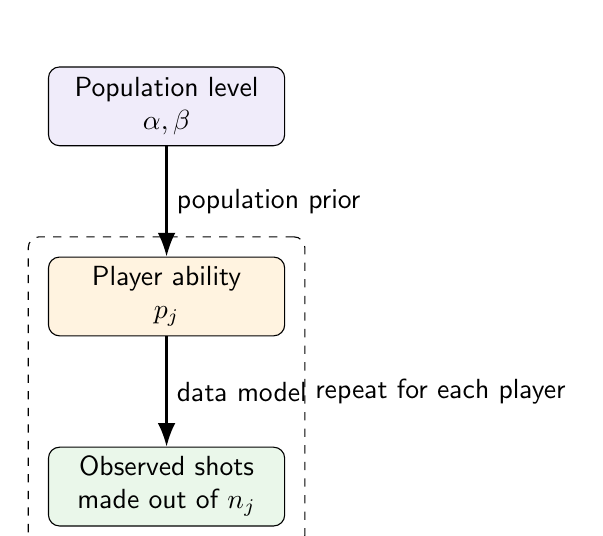
\begin{tikzpicture}[node distance=1.4cm, every node/.style={font=\sffamily}]
  \node[draw, rounded corners, fill=softpurple, minimum width=3.0cm, minimum height=1.0cm, align=center] (ab) {Population level\\$\alpha,\beta$};
  \node[draw, rounded corners, fill=softorange, minimum width=3.0cm, minimum height=1.0cm, align=center, below=of ab] (pj) {Player ability\\$p_j$};
  \node[draw, rounded corners, fill=softgreen, minimum width=3.0cm, minimum height=1.0cm, align=center, below=of pj] (yj) {Observed shots\\made out of $n_j$};
  \draw[-{Latex[length=3mm]}, thick] (ab) -- node[right]{population prior} (pj);
  \draw[-{Latex[length=3mm]}, thick] (pj) -- node[right]{data model} (yj);
  \node[draw, dashed, rounded corners, fit=(pj)(yj), inner sep=0.25cm, label={[font=\sffamily]right:repeat for each player}] {};
\end{tikzpicture}
\end{center}

This kind of model does something useful called \textbf{partial pooling}. A player who took only 2 free throws should not be judged as strongly as a player who took 200. The population distribution gently pulls small-sample estimates toward the group average.

\section{Where do assumptions enter?}

Bayesian inference does not remove assumptions. It makes many assumptions visible.

\begin{checkbox}
For the coin model, important assumptions include:
\begin{enumerate}[leftmargin=1.5em]
  \item \textbf{Same probability:} every flip has the same chance $p$ of heads.
  \item \textbf{Independence:} one flip does not affect the next flip.
  \item \textbf{Correct data recording:} heads and tails are recorded correctly.
  \item \textbf{Chosen prior:} the Beta prior is a reasonable starting description of uncertainty.
  \item \textbf{No hidden changes:} the coin is not switched halfway through the experiment.
\end{enumerate}
\end{checkbox}

In real problems, assumptions are often the hardest part. For example, if you model students' test scores, you might need to think about different teachers, test difficulty, tutoring, missing data, and measurement error.

\begin{bigidea}
A Bayesian answer is conditional on the model. It means: ``Given these assumptions and these data, here is the updated uncertainty.'' If the assumptions change, the posterior can change too.
\end{bigidea}

\section{A second example: measuring a true length}

Suppose a lab group measures the length of a small object. The true length is unknown; call it $\theta$ centimeters. The students measure it five times:

\[
10.1,\quad 9.9,\quad 10.0,\quad 10.2,\quad 9.8.
\]

A simple model might say:

\begin{itemize}[leftmargin=1.5em]
  \item There is one true length $\theta$.
  \item Each measurement equals the true length plus random measurement error.
  \item The errors are usually small, sometimes positive, sometimes negative.
\end{itemize}

In symbols, one common model is:

\[
y_i \sim \operatorname{Normal}(\theta,\sigma).
\]

Here:

\begin{itemize}[leftmargin=1.5em]
  \item $y_i$ is the $i$th measured value.
  \item $\theta$ is the unknown true length.
  \item $\sigma$ describes typical measurement error size.
\end{itemize}

Now ask: what should have a model?

\begin{center}
\begin{tabularx}{\textwidth}{>{\bfseries}p{0.25\textwidth} X}
\toprule
Thing & How to think about it \\
\midrule
The observed measurements $y_i$ & They get a data model: how measurements are generated from the true length. \\
The true length $\theta$ & It is unknown, so it gets a prior. \\
The error size $\sigma$ & If known from the measuring tool, it may be fixed. If unknown, it can get a prior too. \\
The prior settings & If chosen by you, they are fixed hyperparameters. If uncertain and important, they can get higher-level priors. \\
\bottomrule
\end{tabularx}
\end{center}

\section{Posterior predictive thinking}

Once you have a posterior, you can make predictions. This is called the \textbf{posterior predictive distribution}.

For the coin example, after seeing 6 heads and 2 tails with a $\operatorname{Beta}(2,2)$ prior, the posterior is $\operatorname{Beta}(8,4)$. The posterior mean is $8/12\approx 0.667$. A simple prediction for the next flip is therefore about a 66.7\% chance of heads.

But Bayesian prediction also remembers uncertainty. Instead of pretending $p$ is definitely 0.667, it averages over plausible values of $p$ in the posterior.

\begin{center}
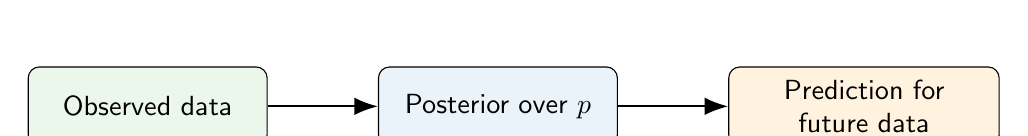
\begin{tikzpicture}[node distance=1.4cm, every node/.style={font=\sffamily}]
  \node[draw, rounded corners, fill=softgreen, align=center, text width=2.8cm, minimum height=1cm] (data) {Observed data};
  \node[draw, rounded corners, fill=lightblue, align=center, text width=2.8cm, minimum height=1cm, right=of data] (posterior) {Posterior over $p$};
  \node[draw, rounded corners, fill=softorange, align=center, text width=3.2cm, minimum height=1cm, right=of posterior] (pred) {Prediction for future data};
  \draw[-{Latex[length=3mm]}, thick] (data) -- (posterior);
  \draw[-{Latex[length=3mm]}, thick] (posterior) -- (pred);
\end{tikzpicture}
\end{center}

\section{A decision guide: what should I model?}

When you feel lost, use this guide.

\begin{recipebox}
\begin{enumerate}[leftmargin=1.5em]
  \item \textbf{What did I observe?} These are the data. Write them as $y$, $x$, or $\data$.
  \item \textbf{What do I want to learn?} These are parameters, such as $p$, $\theta$, or $\mu$.
  \item \textbf{How would the observations be produced if the parameters were known?} This is the likelihood.
  \item \textbf{What did I believe about the parameters before these data?} This is the prior.
  \item \textbf{Are the prior's settings just choices, or are they unknown and important?} If they are just choices, call them fixed hyperparameters. If they are unknown and important, model them too.
  \item \textbf{What assumptions did I make?} Write them down in plain English.
\end{enumerate}
\end{recipebox}

\subsection*{A helpful rule of thumb}

Model something if:

\begin{itemize}[leftmargin=1.5em]
  \item it is unknown,
  \item it matters for the question,
  \item you have data or background knowledge that can tell you something about it,
  \item and ignoring it would make your answer misleading.
\end{itemize}

You do not need to model every detail in the universe. A model is a simplified map. The goal is not to include everything; the goal is to include the important parts for the question you are asking.

\section{Common beginner mistakes}

\begin{warningbox}
\textbf{Mistake 1: Thinking the prior is ``made up'' and therefore useless.}

A prior is an assumption, but all methods use assumptions. Bayesian methods ask you to state this assumption clearly. A weak prior can say, ``I am not very sure.'' A strong prior should only be used when you really have strong background information.
\end{warningbox}

\begin{warningbox}
\textbf{Mistake 2: Thinking the likelihood is automatically true.}

The likelihood is also an assumption. For example, independent coin flips are a model assumption. If the coin is damaged or switched halfway through, the model may be wrong.
\end{warningbox}

\begin{warningbox}
\textbf{Mistake 3: Confusing $P(\data\mid\theta)$ with $P(\theta\mid\data)$.}

$P(\data\mid\theta)$ asks: ``If the parameter had this value, how likely would the data be?''

$P(\theta\mid\data)$ asks: ``After seeing the data, how plausible is this parameter value?''

They are not the same. Bayes' rule connects them.
\end{warningbox}

\begin{warningbox}
\textbf{Mistake 4: Treating the posterior mean as the whole answer.}

The posterior mean is one summary. The full posterior distribution also tells you uncertainty.
\end{warningbox}

\section{Mini practice problems}

\subsection*{Problem 1: Identify the pieces}

A student wants to estimate the chance that a basketball player makes a free throw. The player shoots 20 free throws and makes 14.

\begin{enumerate}[label=(\alph*), leftmargin=1.5em]
  \item What is the observed data?
  \item What is the unknown parameter?
  \item What is a reasonable data model?
  \item What could a prior describe?
\end{enumerate}

\subsection*{Problem 2: Beta update}

Suppose $p\sim\operatorname{Beta}(3,3)$ and you observe 9 heads and 3 tails. What is the posterior?

\subsection*{Problem 3: Hyperparameter or parameter?}

In the model

\[
p\sim\operatorname{Beta}(\alpha,\beta), \qquad y\sim\operatorname{Binomial}(n,p),
\]

which symbol is the main parameter of interest? Which symbols are hyperparameters if they are fixed by the modeler?

\section{Answers to mini practice problems}

\subsection*{Answer 1}

\begin{enumerate}[label=(\alph*), leftmargin=1.5em]
  \item The data are 14 made shots out of 20 attempts.
  \item The unknown parameter is the player's true free-throw probability $p$.
  \item A reasonable simple data model is $y\sim\operatorname{Binomial}(20,p)$, where $y$ is the number of made shots.
  \item A prior describes uncertainty about $p$ before seeing these 20 attempts.
\end{enumerate}

\subsection*{Answer 2}

Use the Beta update rule:

\[
\operatorname{Beta}(\alpha,\beta)+H\text{ heads}+T\text{ tails}
=\operatorname{Beta}(\alpha+H,\beta+T).
\]

So:

\[
\operatorname{Beta}(3,3)+9H+3T=\operatorname{Beta}(12,6).
\]

\subsection*{Answer 3}

The main parameter of interest is $p$, the chance of success. If $\alpha$ and $\beta$ are chosen ahead of time to control the prior for $p$, then $\alpha$ and $\beta$ are fixed hyperparameters.

\section{One-page summary}

\begin{center}
\begin{tabularx}{\textwidth}{>{\bfseries}p{0.26\textwidth} X}
\toprule
Idea & Plain-English meaning \\
\midrule
Bayesian inference & Updating uncertainty after seeing data. \\
Parameter & Unknown quantity you want to learn. \\
Data model / likelihood & A probability model for what data you might see if the parameter were known. \\
Prior & Uncertainty about the parameter before seeing the new data. \\
Posterior & Uncertainty about the parameter after seeing the data. \\
Hyperparameter & A setting that controls a distribution, often the prior. \\
Evidence & The normalizing number that makes the posterior add up to 1. \\
Assumptions & Choices about how the world and measurement process are simplified in the model. \\
\bottomrule
\end{tabularx}
\end{center}

\begin{bigidea}
The most important Bayesian formula is:
\[
P(\theta\mid\data)\propto P(\data\mid\theta)P(\theta).
\]
In words: posterior is proportional to likelihood times prior.
\end{bigidea}

\begin{bigidea}
The most important modeling question is:
\[
\text{What is unknown, and how could the data have been generated from it?}
\]
Answer that clearly, and Bayesian inference becomes much less mysterious.
\end{bigidea}

\end{document}
